\chapter{Introduction}
\label{Chapter5}
\lhead{Chapter 5. \emph{Introduction}}

The exponential growth of data volume has propelled the evolution of multi-gigabit data transmission. This evolution is witnessed not only in wireless but also in wireline communications. The quest for high-speed data transmission brings about a unique set of challenges, one of which is the inherent unpredictability of transmission channel losses.

This demand is further accelerated by the rapid ascent of Artificial Intelligence (AI) and Machine Learning (ML) workloads. The training of Large Language Models (LLMs) requires massive datasets to be moved between distributed computing nodes with minimal latency. Consequently, the ``I/O Wall''—the bottleneck formed by limited interconnect bandwidth—has become a critical hurdle \cite{9269409}. High-speed serial links are no longer just a communication medium; they are the lifeline of modern hyperscale data centers.

To address these bandwidth-hungry applications, the industry is pushing for higher data rates, transitioning from 32 GT/s to 64 GT/s and beyond. This shift necessitates robust equalization and signal integrity measures to recover data over lossy channels, which is the primary focus of this thesis.


\section*{PCIe Standard Overview}

\subsection*{Historical Evolution: From Parallel to Serial}
The architecture of computer systems has evolved dramatically over the last three decades to meet this bandwidth demand.

\subsection*{The Legacy of Parallel PCI}
Early systems relied on the Peripheral Component Interconnect (PCI) bus, a parallel architecture where 32 or 64 bits were transferred simultaneously. While effective for low speeds, parallel buses suffer from clock skew and crosstalk issues that make synchronization impossible at gigahertz frequencies. This physical limitation necessitated the shift to high-speed serial communications.

\subsection*{The Shift to Serial PCIe}
PCI Express (PCIe) abandoned the parallel bus in favor of point-to-point serial links. By embedding the clock within the data stream (Clock and Data Recovery), PCIe eliminated clock skew issues, allowing for scalable frequency increases from Gen 1 (2.5 GT/s) to Gen 6 (64 GT/s).

\begin{figure}[H]
    \centering
    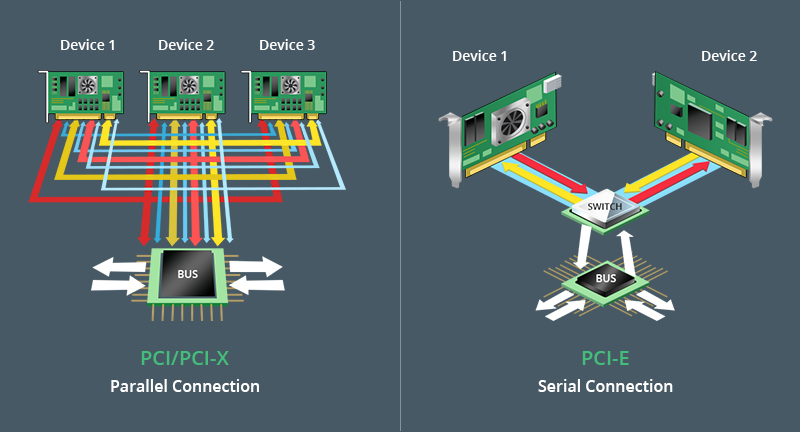
\includegraphics[width=0.5\textwidth]{img/Termination_VGA_img/pcivpcie.png} 
    
    \caption[PCI vs. PCIe Architecture]{Evolution of Bus Architectures: Transition from parallel shared-bus PCI topology to high-speed point-to-point serial PCIe links.}
    \label{fig:pci_vs_pcie}
\end{figure}

\subsection*{Evolution of PCIe}
PCIe has evolved from a simple serial interface to a complex high-performance interconnect. The standard has doubled its data rate approximately every three years while maintaining backward compatibility.

\begin{table}[H]
\centering
\small % Reduces font size slightly for a cleaner look
\begin{tabular}{|l|l|l|l|l|}
\hline
\textbf{Feature} & \textbf{PCIe 3.0} & \textbf{PCIe 4.0} & \textbf{PCIe 5.0} & \textbf{PCIe 6.0} \\ \hline
\textbf{Data Rate} & 8.0 GT/s & 16.0 GT/s & 32.0 GT/s & \textbf{64.0 GT/s} \\ \hline
\textbf{Nyquist Freq} & 4 GHz & 8 GHz & 16 GHz & \textbf{16 GHz} \\ \hline
\textbf{Encoding} & 128b/130b & 128b/130b & 128b/130b & \textbf{1b/1b FLIT} \\ \hline
\textbf{Signaling} & NRZ & NRZ & NRZ & \textbf{PAM4} \\ \hline
\textbf{Unit Interval} & 125 ps & 62.5 ps & 31.25 ps & \textbf{31.25 ps} \\ \hline
\textbf{Channel Loss} & 20 dB & 28 dB & 36 dB & \textbf{32 dB} \\ \hline
\end{tabular}
\caption{Comparative Analysis of PCIe Generations 3.0-6.0}
\label{tab:pcie_generations}
\end{table}

\subsection*{Protocol Architecture}
The PCIe protocol is structured into three primary layers:
\begin{enumerate}
    \item \textbf{Transaction Layer:} Handles TLP assembly and flow control credits.
    \item \textbf{Data Link Layer:} Ensures integrity via LCRC and Sequence Numbers (Ack/Nak).
    \item \textbf{Physical Layer:} Handles the electrical signaling, encoding, and equalization (the focus of this project).
\end{enumerate}

\begin{figure}[H]
    \centering
    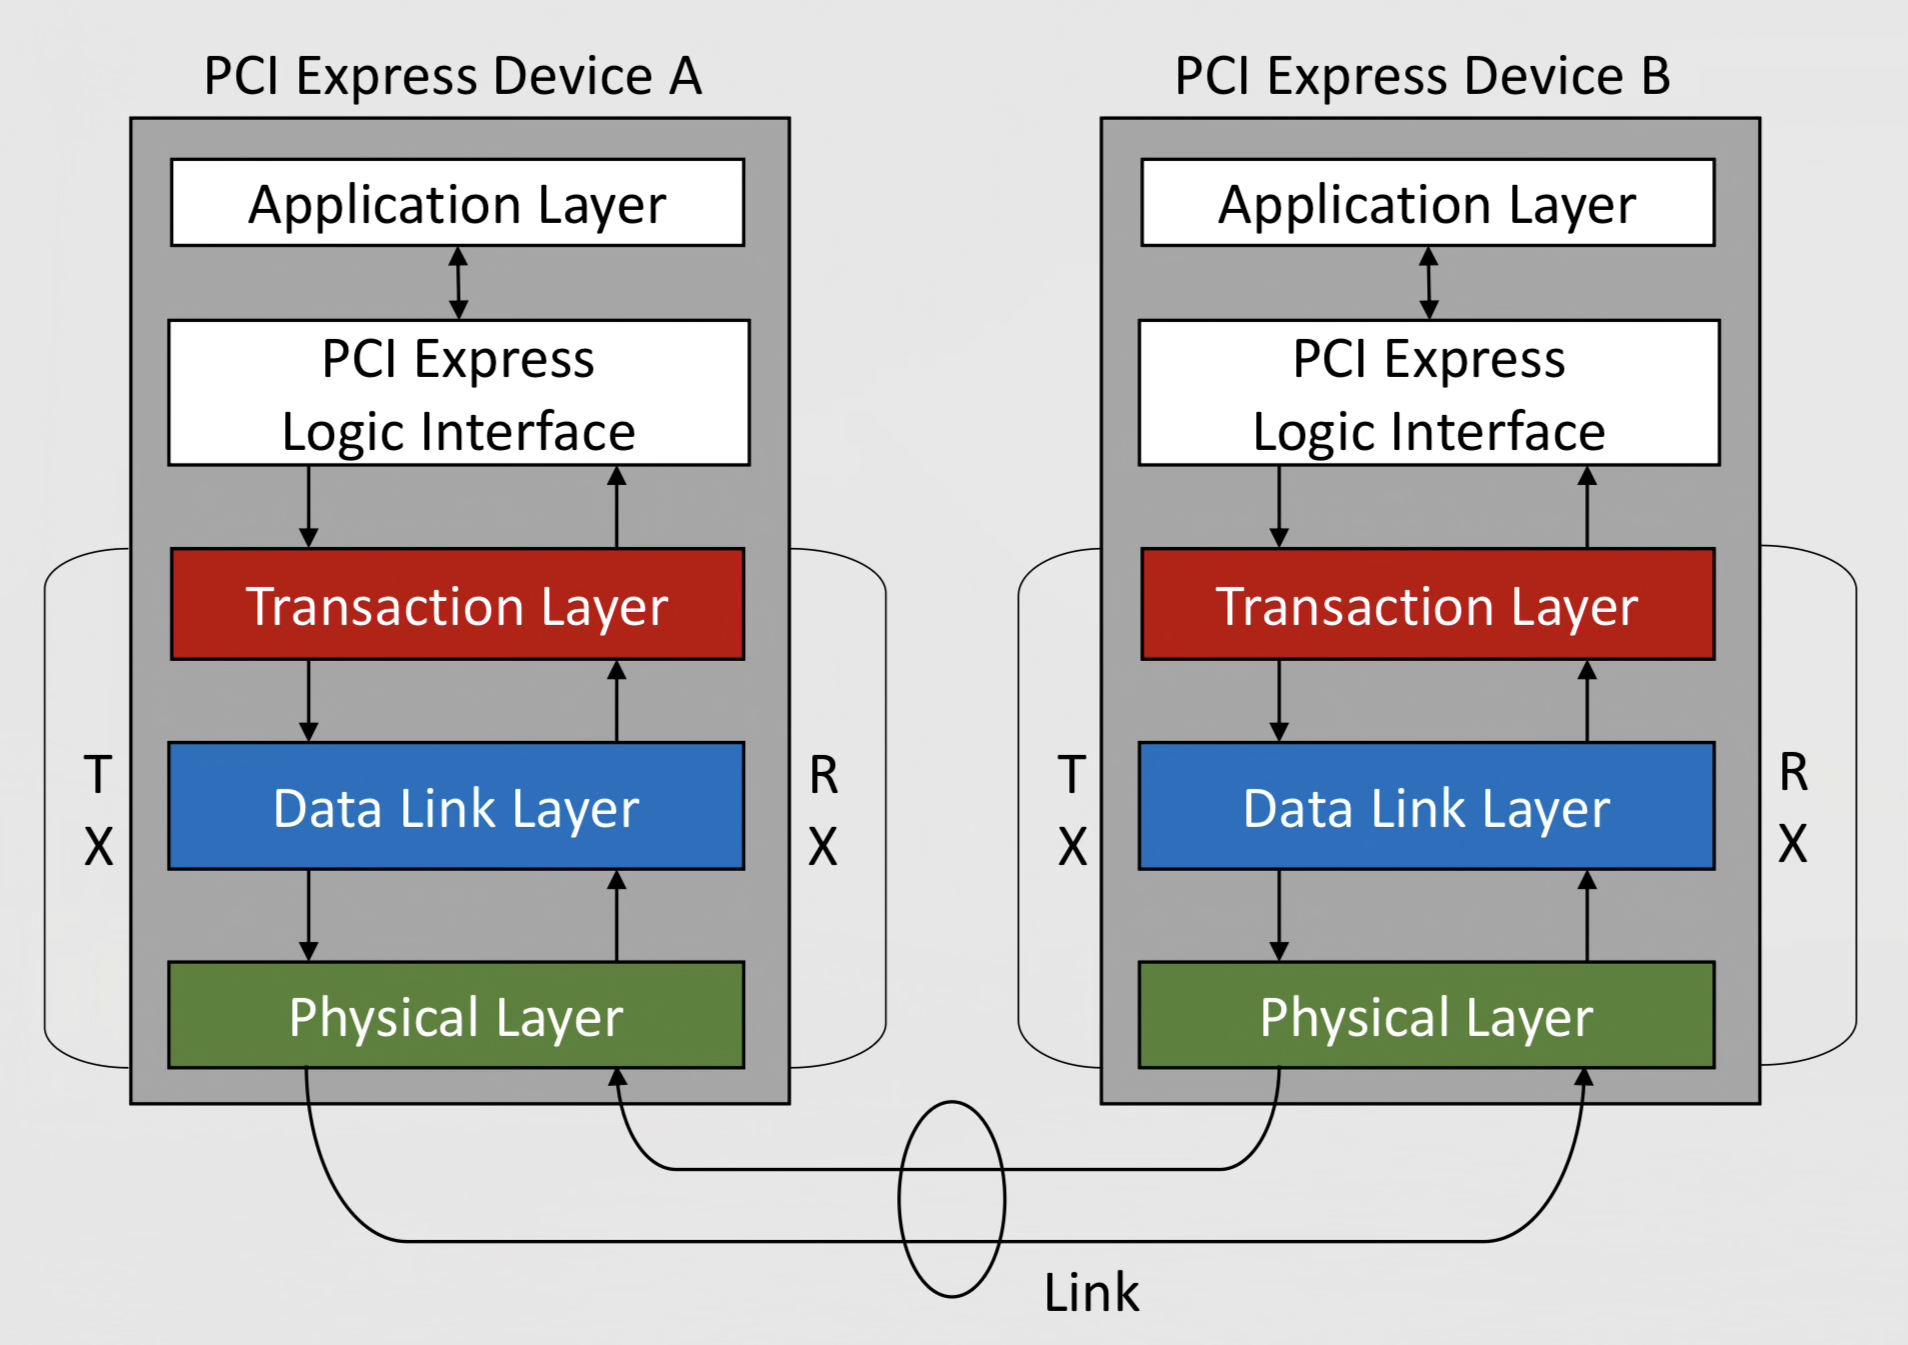
\includegraphics[width=0.5\textwidth]{img/Termination_VGA_img/pciearc.png}
    \caption[PCIe Layer Architecture]{PCIe Protocol Stack and Layer Architecture. (\href{https://www.scribd.com/document/866301752/Introduction-to-PCIe-and-CXL-1746566446}{CERN})}
    \label{fig:pcie_layers}
\end{figure}

\subsection*{PCIe 6.0 Innovations}

\subsection*{PAM4 Signaling}
As shown in Table \ref{tab:pcie_generations}, PCIe 6.0 maintains the 16 GHz Nyquist frequency of Gen 5 but doubles the throughput. This is achieved using Pulse Amplitude Modulation 4-level (PAM4), which encodes 2 bits per symbol.

\begin{figure}[H]
    \centering
    \framebox{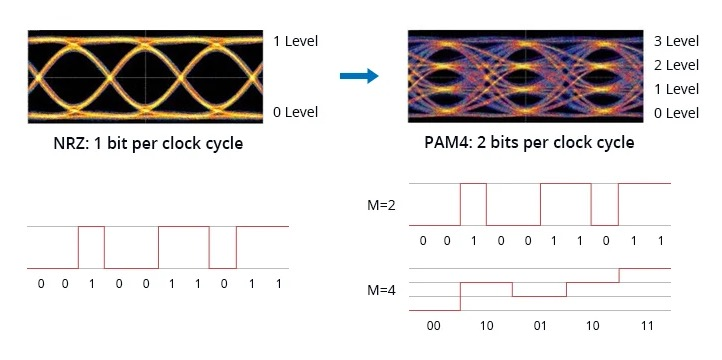
\includegraphics[width=0.7\textwidth]{img/Termination_VGA_img/pam4vnrz.png}}
    \caption[Signaling Comparison]{Comparison of NRZ vs. PAM4 Signaling. (\href{https://www.htfwdm.com/info/what-is-pam4-in-400g-53807632.html}{HTF Future})}
    \label{fig:pam4_nrz}
\end{figure}

\subsubsection*{FLIT Encoding (Flow Control Unit)}
To support the low-latency requirements of high-performance computing, PCIe 6.0 abandons the 128b/130b encoding used in previous generations and adopts \textbf{FLIT Mode (Flow Control Unit)}.

\begin{itemize}
    \item \textbf{Fixed Size:} A FLIT is a fixed-size packet of \textbf{256 Bytes} (64 Double Words).
    \item \textbf{1b/1b Encoding:} Because the FLIT size is fixed and known, the synchronization overhead of 128b/130b is removed. The data is sent with 1b/1b encoding, meaning there is \textbf{zero bandwidth overhead} for encoding, improving spectral efficiency.
    \item \textbf{Structure:} The 256-byte FLIT acts as a container that encapsulates:
    \begin{itemize}
        \item Transaction Layer Packets (TLP) 236B
        \item Data Link Packets (DLP) 6B
        \item Cyclic Redundancy Check (CRC)8B
        \item Forward Error Correction (FEC) 6B
    \end{itemize}
\end{itemize}

\subsubsection*{Forward Error Correction (FEC) and CRC}
Due to the reduced Signal-to-Noise Ratio (SNR) of PAM4, bit errors are more frequent (Target BER $< 10^{-6}$ pre-FEC). PCIe 6.0 implements a robust two-stage error handling mechanism within the FLIT:

\begin{enumerate}
    \item \textbf{Forward Error Correction:} PCIe 6.0 uses a lightweight FEC to correct bit flips without requiring re-transmission. The FEC parity bytes are 3-way interleaved within the FLIT, allowing the receiver to correct specific burst errors that occur due to DFE error propagation within 3 bytes as shown in \ref{fig:flit_structure}.
    
    \item \textbf{Cyclic Redundancy Check:}
    After FEC correction, a dedicated \textbf{CRC} code (separate from the legacy LCRC) is checked.
    \begin{itemize}
        \item If the CRC passes, the FLIT is accepted.
        \item If the CRC fails (meaning the error was too severe for FEC to fix), a Link Layer Retry (LLR) is triggered to re-send the data.
    \end{itemize}
\end{enumerate}

This combination ensures that the final bit error rate remains phenomenally low (FIT $< 10^{-9}$), equivalent to previous NRZ generations, despite the fragility of PAM4 signaling.

\section*{Thesis Organization}
This thesis is organized as follows:
\begin{itemize}
    \item \textbf{Chapter \ref{Chapter2}} presents the system overview and theoretical foundation of the PCIe interface.
    \item \textbf{Chapter \ref{Chapter3}} details the literature survey and architecture selection for the complete receiver system.
    \item \textbf{Chapter \ref{Chapter4}} details the proposed circuit implementation of the Receiver.
    %\item \textbf{Chapter \ref{Chapter5}} presents the post-layout simulation results.
    %\item \textbf{Chapter \ref{Chapter6}} concludes the work and discusses future directions.
\end{itemize}